\section{System Performance Evaluation}
\label{kvdirect:sec:eval}
\label{kvdirect:sec:evaluation}
\label{kvdirect:sec:system-benchmark}

\subsection{System Implementation}

To improve development efficiency, Intel FPGA SDK for OpenCL~\cite{aoc} is used to synthesize the hardware logic of OpenCL. The key-value processor is implemented with 11,000 lines of OpenCL code, all kernels are fully pipelined, that is, the throughput is one operation per clock cycle. With a clock frequency of 180~MHz, key-value operations can be processed at 180~M op/s, if the network, DRAM, or PCIe is not a bottleneck.

%\textbf{Network protocol, client}

\subsection{Testbed and Evaluation Method}

This section evaluates KV-Direct on a testbed of 8 servers and 1 Arista DCS-7060CX-32S switch. Each server is equipped with two 8-core Xeon E5-2650 v2 CPUs with hyperthreading disabled, forming two NUMA nodes connected by QPI Link. Each NUMA node is equipped with 8 DIMM 8~GiB Samsung DDR3-1333 ECC RAM, with a total of 128~GiB of host memory on each server. The programmable network card~\cite{caulfield2016cloud} is connected to the PCIe root complex of CPU 0, and its 40~Gbps Ethernet port is connected to the switch. The programmable network card has two PCIe Gen3 x8 links in the bifurcated Gen3 x16 physical connector. The tested server is equipped with a SuperMicro X9DRG-QF motherboard and a 120~GB SATA SSD running Archlinux (kernel version 4.11.9-1).

For system benchmarking, the YCSB workload \cite{cooper2010benchmarking} is used. For skewed Zipf workloads, this paper selects a skewness of 0.99 and refers to it as a \textit{long-tail} workload.

Before each benchmark, the hash index ratio, inline threshold, and load distribution ratio are adjusted according to the key-value size, access pattern, and target memory utilization. Then, random key-value pairs of a given size are generated. The key size for a given inline key-value size is irrelevant to the performance of KV-Direct, as the keys are padded to the longest inline key-value size during processing. For testing inline cases, the key-value size is used as a multiple of the slot size (when the size is $\leq$ 50, i.e., 10 slots). For testing non-inline cases, the key-value size used is a power of 2 minus 2 bytes (for metadata). As the final step of preparation, PUT operations are issued to insert the key-value pairs into the free key-value storage until 50\% memory utilization. Performance under other memory utilizations can be obtained from Figure \ref{kvdirect:fig:mem-access-tput}.

During the benchmark, a FPGA-based packet generator \cite{li2016clicknp} is used in the same ToR to generate batches of key-value operations, send them to the key-value server, receive completions, and measure sustainable throughput and latency. The processing latency of the packet generator is pre-calibrated by direct loopback and removed from the latency measurement. The error lines represent the $5^{th}$ and $95^{th}$ percentiles.

\subsection{Throughput}

Figure \ref{kvdirect:fig:ycsb-tput} shows the throughput of KV-Direct under YCSB uniform and long-tail (skewed Zipf) workloads. Three factors may be bottlenecks for KV-Direct: clock frequency, network, and PCIe/DRAM. For 5B to 15B key-values inlined in the hash index, most GETs require one PCIe/DRAM access, while PUTs require two PCIe/DRAM accesses. These small key-values are common in many systems. In PageRank, the key-value size of edges is 8B. In sparse logistic regression, the key-value size is typically 8B-16B. For sequencer programs and locks in distributed systems, the key-value size is 8B.

\begin{figure}[htbp]
	\centering
	\subfloat[Uniform distribution.\label{kvdirect:fig:ycsb-tput-uniform}]
	{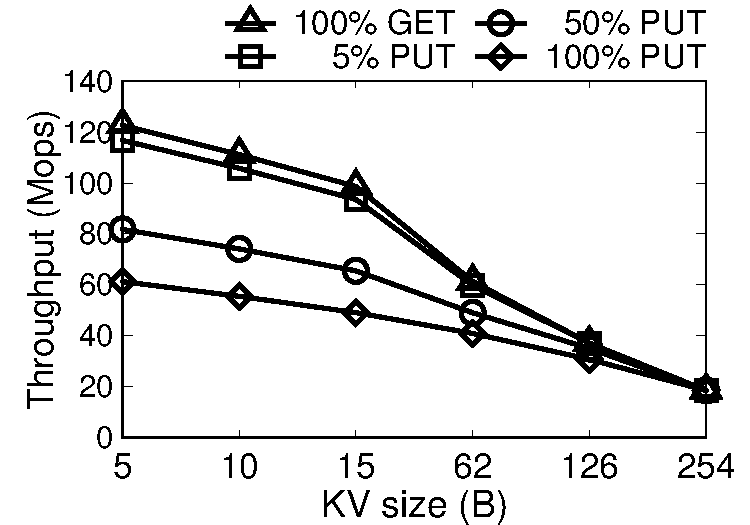
\includegraphics[width=.5\textwidth,page=1]{ycsb-tput-uniform.pdf}}
	\subfloat[Long-tail distribution.\label{kvdirect:fig:ycsb-tput-longtail}]
	{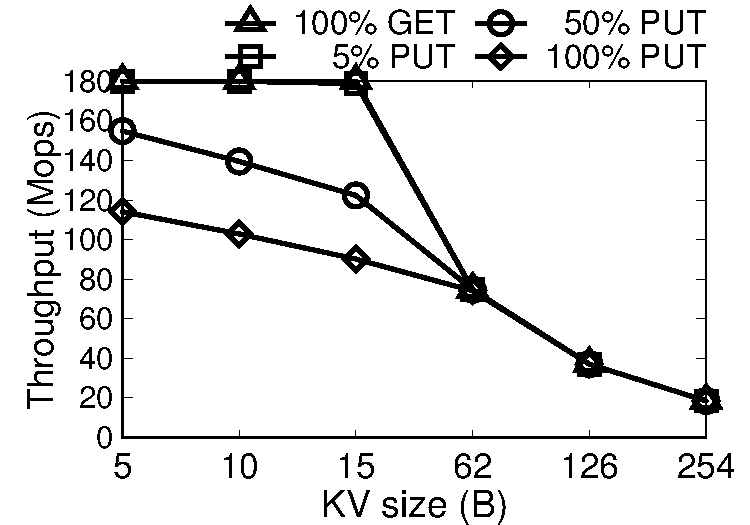
\includegraphics[width=.5\textwidth,page=1]{ycsb-tput-longtail.pdf}}
	\caption{Throughput of KV-Direct under YCSB workloads.}
	\label{kvdirect:fig:ycsb-tput}
\end{figure}

At the same memory utilization, larger inline key-values have lower throughput due to a higher probability of hash collisions. Key-values of 62B and larger are not inlined, so they require additional memory accesses. The long-tail workload has higher throughput than the uniform workload and can reach the clock frequency range of 180~Mops under read-intensive workloads, or reach the network throughput of $\geq$ 62B key-value sizes. Under the long-tail workload, the out-of-order execution engine merges about 15\% of operations on the most popular keys, and the on-board DRAM has about a 60\% cache hit rate at a 60\% load distribution ratio, which can result in up to 2x the throughput as a uniform workload. As shown in Table \ref{kvdirect:tab:kvs-compare}, the throughput of the KV-Direct network card is comparable to that of state-of-the-art key-value storage servers with dozens of CPU cores.

\begin{sidewaystable}[htbp]
	\centering
	\caption{Comparison of KV-Direct with other key-value storage systems under long-tail (skewed Zipf) load and 10-byte small keys. For performance numbers not reported in related work, this paper simulates these systems using similar hardware and reports rough measurement results. For CPU bypass systems, the numbers in parentheses report the difference in power consumption under peak load and idle conditions.}
	\label{kvdirect:tab:kvs-compare}
	\small
	\begin{tabular}{|l|l|l|r|r|r|r|r|r|r|}
		\toprule
		Key-value storage  & Note & Performance bottleneck & \multicolumn{2}{c|}{Throughput (Mops)} & \multicolumn{2}{c|}{Power efficiency (Kops/W)} & \multicolumn{2}{c|}{Average latency ($\mu$s)} \\
		\cline{4-9}Table \ref {clicknp:tab:elements} 
		& & & GET & PUT & GET & PUT & GET & PUT \\
		\midrule
		Memcached~\cite{fitzpatrick2004distributed} & Traditional & Inter-core CPU synchronization & 1.5 & 1.5 & \approx5 & \approx5 & \approx50 & \approx50 \\
		MemC3~\cite{fan2013memc3} & Traditional & Operating system network protocol stack & 4.3 & 4.3 & \approx14 & \approx14 & \approx50 & \approx50 \\
		RAMCloud~\cite{ousterhout2015ramcloud} & Kernel bypass & Dispatch thread & 6 & 1 & \approx20 & \approx3.3 & 5 & 14 \\
		MICA~\cite{lim2014mica} & Kernel bypass, 24 cores, 12 NIC ports & CPU key-value processing & 137 & 135 & 342 & 337 & 81 & 81 \\
		FaRM~\cite{dragojevic2014farm} & One-sided RDMA GET & RDMA NIC & 6 & 3 & \approx30 (261) & \approx15 & 4.5 & \approx10 \\
		DrTM-KV~\cite{wei2015fast} & One-sided RDMA and HTM & RDMA NIC & 115.2 & 14.3 & \approx500 (3972) & \approx60 & 3.4 & 6.3 \\
		HERD'16~\cite{kalia2016design} & Two-sided RDMA, 12 cores & PCIe & 98.3 & \approx60 & \approx490 & \approx300 & 5 & 5 \\
		Xilinx'13~\cite{blott13hotcloud} & FPGA & Network & 13 & 13 & 106 & 106 & 3.5 & 4.5 \\
		Mega-KV~\cite{zhang2015mega} & GPU (4~GiB on-board RAM) & GPU key-value processing & 166 & 80 & \approx330 & \approx160 & 280 & 280 \\
		\midrule
		\textbf{KV-Direct (1 NIC)} & Programmable NIC, two Gen3 x8 & PCIe \& DRAM & 180 & 114 & 1487 (5454) & 942 (3454) & 4.3 & 5.4 \\
		\textbf{KV-Direct (10 NICs)} & Programmable NIC, one Gen3 x8 per card & PCIe \& DRAM & 1220 & 610 & 3417 (4518) & 1708 (2259) & 4.3 & 5.4 \\
		\bottomrule
	\end{tabular}
\end{sidewaystable}


\subsection{Power Efficiency}

Inserting the KV-Direct NIC can add 10.6 W of power to an idle server.
When the KV-Direct server is at peak throughput, the system power is 121.4 watts (measured at the wall).
Compared with the most advanced key-value storage systems in Table \ref {kvdirect:tab:kvs-compare}, the power efficiency of KV-Direct is three times that of other systems, and it is the first to reach one million key-value operations per watt on a commercial server.

When the KV-Direct NIC is unplugged, the power consumption of the idle server is 87.0 watts, so the total power consumption of the programmable NIC, PCIe, host memory, and daemon on the CPU is only 34 watts.
The measured power difference is reasonable because the CPU is almost idle, and the server can run other workloads while KV-Direct is running (using the same standard for one-sided RDMA, as shown in parentheses in Table \ref{kvdirect:tab:kvs-compare}).
In this respect, the power efficiency of KV-Direct is ten times that of CPU-based systems.

\subsection{Latency}

Figure \ref {kvdirect:fig:ycsb-lat} shows the latency of KV-Direct under peak YCSB workload throughput. Without network batching, the tail latency ranges from 3 to 9 $\mu$s, depending on the key-value size, operation type, and key distribution. Due to the additional memory access, PUT has a higher latency than GET. Skewed workloads have lower latency than uniform ones because they are more likely to be cached in on-board DRAM. Larger key-values have higher latency due to the additional network and PCIe transfer latency. Network batching adds less than 1~$\mu$s of latency compared to non-batching operations, but significantly improves throughput, as evaluated in Figure \ref {kvdirect:fig:eval-network-batching}.

\begin{figure}[htbp]
	\centering
	\subfloat[With batching.\label{kvdirect:fig:ycsb-lat-batch}]
	{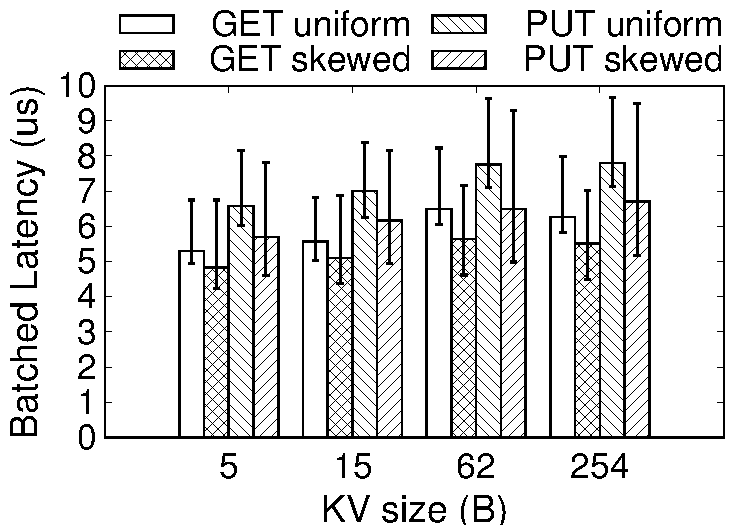
\includegraphics[width=.5\textwidth,page=1]{lat-batch.pdf}}
	\subfloat[Without batching.\label{kvdirect:fig:ycsb-lat-nobatch}]
	{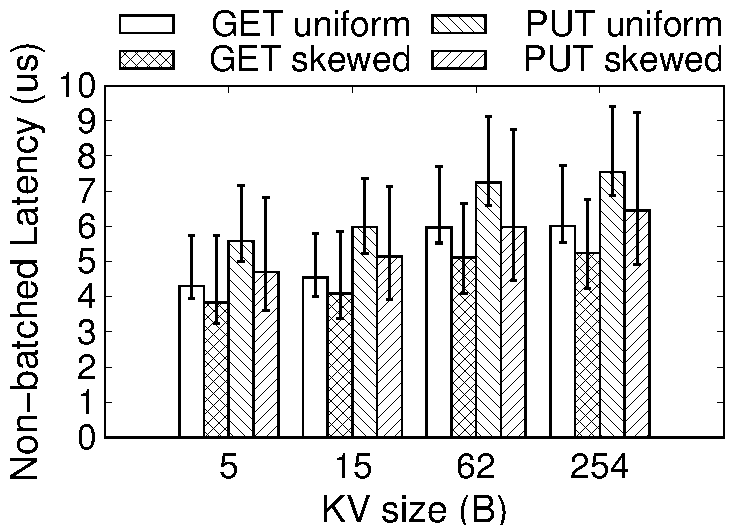
\includegraphics[width=.5\textwidth,page=1]{lat-nonbatch.pdf}}
	\caption{Latency of KV-Direct under peak YCSB workload throughput.}
	\label{kvdirect:fig:ycsb-lat}
\end{figure}

\subsection{Impact on CPU Performance}

KV-Direct aims to bypass the server CPU, using only a portion of host memory for key-value storage. Therefore, the CPU is still available to run other applications. When a single NIC KV-Direct is at peak load, the measured impact on other workloads on the server is minimal. Table \ref {kvdirect:tab:cpu-impact} quantifies the impact of KV-Direct peak throughput. Except for the sequential throughput of CPU 0 to access its own NUMA memory (rows marked in bold), the latency and throughput of CPU memory access are mostly unaffected. This is because the 8 host memory channels can provide higher random access throughput than all CPU cores can consume, while the CPU can indeed stress the sequential throughput of the DRAM channels. The impact of the host daemon process is minimal when the distribution of key-value sizes is relatively stable, as the garbage collector is only invoked when the number of available slots for different board sizes is unbalanced.

\begin{table}[htbp]
	\centering
	\caption{Impact on CPU memory access performance when KV-Direct is at peak throughput. Measured using Intel Performance Counter Monitor (Intel PCM) V2.11.}
	\label{kvdirect:tab:cpu-impact}
	\small
		\begin{tabular}{l|l|r|r}
			\toprule
			\multicolumn{2}{r}{KV-Direct Status $\rightarrow$} & Idle & Busy \\
			\midrule
			\multirow{4}{*}{\specialcell{Random Access Latency}} & CPU0-0 & 82.2 ns & 83.5 ns \\
            					  & CPU0-1 & 129.3 ns & 129.9 ns \\
                                  & CPU1-0 & 122.3 ns & 122.2 ns \\
                                  & CPU1-1 & 84.2 ns & 84.3 ns \\
			\midrule
            \multirow{4}{*}{\specialcell{Sequential Access Throughput}} & \textbf{CPU0-0} & \textbf{60.3 GB/s} & \textbf{55.8 GB/s} \\
            					  & CPU0-1 & 25.7 GB/s & 25.6 GB/s \\
                                  & CPU1-0 & 25.5 GB/s & 25.9 GB/s \\
                                  & CPU1-1 & 60.2 GB/s & 60.3 GB/s \\
			\midrule
			\multirow{4}{*}{\specialcell{Random Access Throughput}} & 32B Read & 10.53 GB/s & 10.46 GB/s \\
            						& 64B Read & 14.41 GB/s & 14.42 GB/s \\
                                    & 32B Write & 9.01 GB/s & 9.04 GB/s \\
                                    & 64B Write & 12.96 GB/s & 12.94 GB/s \\
			\bottomrule
		\end{tabular}      
\end{table}

